%Use RevTex 4.2
\documentclass[aps,pra,reprint]{revtex4-2}
\usepackage{graphicx}
\usepackage{amsmath}
\usepackage[T1]{fontenc}
\usepackage[utf8]{inputenc}
\usepackage{hyperref}

\bibliographystyle{apsrev4-2}

\begin{document}

\title{Statistical properties of cold bosons in a ring trap}
\date{\today}

\author{Maciej Kruk}
\affiliation{Center for Theoretical Physics, Polish Academy of Sciences, Aleja
 Lotników 32/46, 02-668 Warsaw, Poland}

\author{Maciej Łebek}
\email{mlebek@cft.edu.pl}
\affiliation{Center for Theoretical Physics, Polish Academy of Sciences, Aleja
 Lotników 32/46, 02-668 Warsaw, Poland}

\author{Kazimierz Rzążewski}
\affiliation{Center for Theoretical Physics, Polish Academy of Sciences, Aleja
 Lotników 32/46, 02-668 Warsaw, Poland}

\begin{abstract}
A study of an interacting system of bosons in a ring trap at a finite 
temperature is presented. We consider a gas with contact and long-range dipolar 
interactions within a framework of the classical fields approximation. For a 
repulsive gas we have obtained coherence length, population of the ground state 
and its fluctuations as a function of temperature. In the case of an attractive 
gas we study local density fluctuations.  Additionally, we exactly calculate 
the partition function for the ideal gas in the canonical ensemble and derive 
several other macroscopic state functions.
\end{abstract}

\maketitle

\section{Introduction}\label{intro}
The physics of Bose-Einstein condensation has been intensively studied since 
the appearance of the first papers published in the 1920s~\cite{Bose1924,
*Einstein1924,*Einstein1925}. Theoretical research investigated not only 
population of the condensate, but also its fluctuations. The problem of the 
latter turned out to be more troublesome. E. Schr{\"o}dinger was the first 
to observe that the standard theory of noninteracting gas in the grand 
canonical ensemble predicts unphysically large fluctuations 
~\cite{Schrodinger1989}. Later on, it was noted that different 
fluctuations are found in different statistical ensembles~\cite{Ziff1977}.
    
The new era of BEC studies began in 1995, when the rubidium and sodium gases 
were condensed in laboratories~\cite{Davis1995,*Anderson1995}. Not 
surprisingly, that achievement accelerated the progress of theory. Papers 
concerning canonical~\cite{Politzer1996} and microcanonical~\cite{Navez1997} 
ensemble fluctuations in the experimentally relevant case of the harmonic trap 
appeared shortly after. These results were followed by studies of interacting 
gases in the later years
~\cite{Bienias2011c,Bienias2011b,Bhattacharyya2016,Idziaszek1999}. It is worth 
stressing that there are still many open questions in this area, e.g. results 
are inconclusive, for details see~\cite{Kristensen2019}.
    
Over ten years ago, local density fluctuations of quasi-1D Bose gas were 
measured ~\cite{Esteve2006}. However, until now, there were no experimental 
data concerning fluctuations of the population of the condensate. The recent 
pioneering measurements of fluctuations~\cite{Kristensen2019} revive the 
interest in such problem in the case of weakly interacting Bose gas.
    
In this paper, we present detailed studies of statistical properties of the 
interacting Bose gas confined to a toroidal trap. Such a confinement makes 
the system effectively one-dimensional. A trap of that form has been 
succesfully realized in experiment ~\cite{Ramanathan2011}.
     
We analyze two types of interaction between particles: contact and dipolar 
long-range ones as defined in~\cite{Sinha2007}.
For dipolar interaction, both attractive and repulsive character can be 
achieved. In case of the repulsive interactions, we study number of atoms 
in the condensate and its fluctuations as a function of temperature. 
Additionally, we analyze the impact of temperature on a coherence length. 
For an attractive case, i.e. in the presence of bright solitons, we investigate 
local density fluctuations. Results concerning interacting system are supported 
by exact analytic expressions for the ideal gas obtained in the canonical 
ensemble. We consider system with number of particles equal $N=100$. 
     
Paper is structured in the following way.  In Sec.~\ref{model} we present 
the most important theoretical aspects of our model that are common to all 
problems that we adress and discuss our main methods using which we obtain 
macroscopic state functions of the gas. Sec.~\ref{repulsive} and 
Sec.~\ref{attractive} are dedicated exclusively to theoretical extensions 
of our model and results concerning repulsive and attractive gas. Paper 
is ended with a brief summary in Sec.~\ref{summary} containing the most 
important conclusions of our work. In the Appendix we present analytic formulas 
for partition function, correlation function and fluctuations of the zero 
momentum component for the ideal gas in the canonical ensemble.

\section{The model}\label{model}
The Hamiltonian of the system we consider in this paper reads
\begin{equation}
\label{eq:hamiltonian}
\begin{split}
\hat{H} & = \int \mathrm{d}x \; {\hat{\psi}}^{\dag}(x) \frac{\hat{p}^2}{2m} 
\hat{\psi}(x) + \\
& + \int \int \mathrm{d}x \, \mathrm{d}x' \; {\hat{\psi}}^{\dag}(x) 
{\hat{\psi}}^{\dag}(x') \hat{V}(x-x') \hat{\psi}(x') \hat{\psi}(x)
\end{split}
\end{equation}
with $\hat{p}$ - momentum operator, $m$ - mass of the particle 
and $\hat{V}(x-x')$ - interaction potential.
    
In order to cope with the difficult problem of interacting particles, we employ 
the classical fields approximation. It consists of replacing the atomic field 
operator $\hat{\psi}(x)$ by a complex c-number function $\psi(x)$ 
(for details see~\cite{Brewczyk2007}). We can tune it to give us correct 
macroscopic state functions, provided we choose the optimal momentum cutoff. 
The use of such an approximation is analogous to using Maxwell equations 
instead of QED in the case of light, for which a cutoff is necessary to avoid 
the UV catastrophe known in the theory of black-body radiation.
    
The main idea behind the classical fields approximation is to replace creation 
and annihilation operators by complex amplitudes and to neglect modes with 
value of momentum higher than cutoff momentum $k_{max}$. The problem of 
choosing the proper value of the cutoff is discussed in detail in repulsive 
and attractive gas sections. 
    
In this paper we rely on mathematical equivalence between particles on the ring 
and free particles with periodic boundary conditions with period equal to 
the length of the trap $L$. The atomic field within the classical fields 
approximation
\begin{equation}
\psi(x) = \sum_{-k_{max}}^{k_{max}} \alpha_k \, \varphi_k(x) =
\sum_{-k_{max}}^{k_{max}} \frac{1}{\sqrt{L}} \, \alpha_k \, e^{i k x},
\end{equation}
where the set $\varphi_k$ is the orthonormal basis in the single-particle 
Hilbert space and $k=\frac{2 \pi n}{L}, \, n=0, \pm 1, \ldots , \pm n_{max}$. 
Energy corresponding to state $\varphi_k$ is equal 
$E_k = \frac{\hbar ^2 k^2}{2m}=\frac{2 \pi ^2 \hbar ^2}{m L^2} n^2$. From now 
we will use $\epsilon \equiv \frac{2 \pi ^2 \hbar ^2}{m L^2}$, 
$\hbar/ \epsilon$ and $L$ as units of energy, time and length respectively. 
Hamiltonian as a function of the complex amplitudes $\alpha_j$ reads
\begin{equation}
\label{Halpha}
H = \sum_{-n_{max}}^{n_{max}} j^2 |\alpha_j|^2 + \frac{1}{2} 
\sum_{j_1,j_2,j_3,j_4} C_{j_1,j_2,j_3,j_4} \, \alpha^*_{j_1} \alpha^*_{j_2} 
\alpha_{j_3} \alpha_{j_4},
\end{equation}
where
\begin{equation}
\begin{split}
&C_{j_1,j_2,j_3,j_4} = \\ 
& = \int_0^{1} \int_0^{1} \mathrm{d}x \, \mathrm{d}x' \; 
e^{-2 \pi i[(j_1-j_3)x+(j_2-j_4)x']} \; V(x-x').
\end{split}
\end{equation}
Additionally, we obtain set of equations of motion for amplitudes $\alpha _j$. 
Plugging Hamiltonian~\eqref{eq:hamiltonian} into the Heisenberg equation and 
replacing operators with complex amplitudes yields
\begin{equation}
\label{eq:eqs}
i \, \frac{\mathrm{d} \alpha_j}{\mathrm{d} t} = j^2 \alpha_j + 
\sum_{j_1,j_2,j_3} C_{j_1,j,j_2,j_3} \, \alpha^*_{j_1} \alpha_{j_2} 
\alpha_{j_3},
\end{equation}
where $j=0, \pm 1, \ldots ,\pm n_{max}$.
    
We consider contact interparticle potential $V(x-x')=g \, \delta(x-x')$ and 
quasi-1D dipole-dipole interaction potential~\cite{Deuretzbacher2010}
\begin{equation}
\begin{split}
&V(x-x') = g \; \frac{1}{4 l_{\perp}} \Bigglb (-2\Big|\frac{x-x'}{l_{\perp}}\Big| +
\\ 
& + \sqrt{2 \pi} \, \bigg(1 + \Big|\frac{x-x'}{l_{\perp}}\Big|^2 \bigg) \, 
e^{\frac{1}{2}\big|\frac{x-x'}{l_{\perp}}\big|^2} 
\text{Erfc} \Bigg(\Big|\frac{x-x'}{\sqrt{2}l_{\perp}}\Big|\Bigg)\Biggrb )
\end{split}
\end{equation}
with dependence on $l_{\perp}=\sqrt{\frac{\hbar}{m \omega _{\perp}}}$, 
where $\omega _{\perp}$ is the frequency of harmonic trap responsible for 
transversal confinement of particles. Note that length $l_{\perp}$ is directly 
related to the width of the dipolar potential and the potential is normalized 
to the parameter $g$ quantifying the strength of the interactions
~\cite{Deuretzbacher2010}. In our model the parameter $g$ is determined by two 
factors: dipole moments and their orientation which is kept constant during 
motion of the particles. By proper orientation of dipoles on the ring we are 
able to obtain attractive ($g<0$) and repulsive ($g>0$) character of 
interactions. For $x \gg 0$ we observe $ V(x) \sim \frac{1}{x^3}$ 
as for the standard dipolar potential.
     
The full formula for quasi-1D potential contains additional 
$\delta$-interaction term~\cite{Sinha2007}. However, we want to focus on 
differences between short and long-range interactions, that is why we consider 
the situation where this term can be neutralized. One can achieve this by 
proper tuning of Feshbach resonances leading 
to the cancellation of $\delta$ terms.
    
Due to the ring geometry or equivalently, periodic boundary conditions, the 
expression for long-range potential should be 
modified~\cite{*[{ }] [{ - Appendix }] Odziejewski2018}
\begin{equation}
V_{per}(x-x') = \sum_{n=-\infty}^{\infty} V(x-x'-n).
\end{equation}

In this paper we will use canonical ensemble for a system described with 
the classical fields approximation. To obtain estimates of statistical 
properties, we sample the ensemble with a Monte Carlo (MC) algorithm.
     
First, to get the states from the thermal equilibrium distribution of the 
canonical ensemble we decided to use Metropolis algorithm \cite{Metropolis1953} 
implemented as described in~\cite{Witkowska2010} with code available 
here~\footnote{\url{github.com/mbkruk/BoseGas}}. We compare these results to 
those  obtained from the time evolution of equations~\eqref{eq:eqs}.
    
The equations of motion~\eqref{eq:eqs} look similar to those studied by Fermi, 
Pasta and Ulam~\cite{Fermi1955}. For contact interactions they can be seen as 
set of equations describing evolution of Fourier amplitudes of function 
$\psi(x)$ satisfying periodic nonlinear Schr{\"o}dinger equation (NLS). It is 
known that periodic NLS have an infinite number of constants of 
motion~\cite{Faddeev2007}. It means that in principle our system is not 
ergodic. Three constants of motion have clear interpretation of energy, 
momentum and the number of particles. That is why we can think of time-averaged 
quantities as quantities obtained in a microcanonical ensemble further 
constrained by the constant momentum and the remaining constants of motion. 
Note that for the ideal gas ($g=0$) evolution given by~\eqref{eq:eqs} leads to 
occupations of modes that are constant in time hence equations~\eqref{eq:eqs} 
are not adequate to describe time evolution of noninteracting system.

\section{The repulsive gas}\label{repulsive}
As indicated in the introduction, this section covers two independent subjects: 
population of the condensate together with its fluctuations and coherence 
length. Each one of these two problems requires a different choice of the 
cutoff parameter. That aspect of classical fields approximation - the need to 
change the cutoff to obtain correct values of different state functions, was 
discussed in detail in the paper~\cite{Pietraszewicz2018}.  In both situations 
our point of reference to establish criterion for cutoff are exact results for 
the ideal gas in the canonical ensemble.

\subsection{Population of the condensate and its fluctuations}
We start this section with discussion of the cutoff parameter $n_{max}$ which 
plays an important role in our calculations. To determine its optimal value, 
we use similar approach to~\cite{Witkowska2009,Witkowska2010}. We turn to 
noninteracting gas of $N$ bosons and calculate probability distribution 
$P(N_{ex})$  of having $N_{ex}$ atoms excited~\eqref{eq:Pexact}. We use the 
canonical ensemble and compare our results to similar distribution 
$P_{cl}(N_{ex})$ which has the same physical meaning but is obtained using 
classical fields approximation~\eqref{eq:Pclass}. For more details see the 
Appendix, where we derive formulas~\eqref{eq:Pexact} and~\eqref{eq:Pclass}. We 
introduce standard notation $\beta=1/k_{\textit{B}} T$.
\begin{widetext}
\begin{equation}
\label{eq:Pexact}
P(N_{ex}) = \frac{\sum_{j=1}^{\infty} e^{-\beta E_j N_{ex}} 
\prod_{\substack{k=1 \\ k \neq j}}^{\infty} \frac{1}{(1-e^{-\beta(E_k-E_j)})^2} 
\bigg(N_{ex} + 1 + 2\sum_{\substack{l=1 \\ l \neq j}}^{\infty} 
\frac{1}{1-e^{-\beta(E_j-E_l)}} \bigg)}
{\prod _{j=1}^{\infty} \frac{1}{(1-e^{-\beta E_j})^2} - 
\sum_{j=1}^{\infty}\frac{e^{-\beta E_j N}}{e^{ \beta E_j}-1} 
\prod_{\substack{k=1 \\ k \neq j}}^{\infty} \frac{1}{(1-e^{-\beta(E_k-E_j)})^2} 
\bigg(N + 1 + \frac{1}{1-e^{-\beta E_j}} + 
2\sum_{\substack{l=1 \\ l \neq j}}^{\infty} 
\frac{1}{1-e^{-\beta(E_j-E_l)}} \bigg)}
\end{equation}
\begin{equation}
\label{eq:Pclass}
P_{cl}(N_{ex}) = \frac{\sum_{j=1}^n e^{-\beta E_j N_{ex}} 
\prod_{\substack{k=1 \\ k \neq j}}^n \frac{1}{(\beta E_k-\beta E_j)^2} 
\bigg(N_{ex} + 2\sum_{\substack{l=1 \\ l \neq j}}^n 
\frac{1}{\beta E_j-\beta E_l}\bigg)}
{\prod_{j=1}^n \frac{1}{(\beta E_j)^2} - 
\sum_{j=1}^n \frac{e^{-\beta E_j N}}{\beta E_j} 
\prod_{\substack{k=1 \\ k \neq j}}^n \frac{1}{(\beta E_k-\beta E_j)^2}
\bigg(N + \frac{1}{\beta E_j} + 2\sum_{\substack{l=1 \\ l \neq j}}^n 
\frac{1}{\beta E_j-\beta E_l}\bigg)}
\end{equation}
\end{widetext}

Continous distribution~\eqref{eq:Pclass} is discretized. We do that by dividing 
the interval $[0,N]$ into $N+1$ subintervals of equal size and averaging the 
distribution over subsequent subintervals. Optimal cutoff corresponds to the 
situation, where two distributions:  exact and discretized classical match each 
other (in Fig. \ref{fig:comp} we show an example).    
\begin{figure}[h]
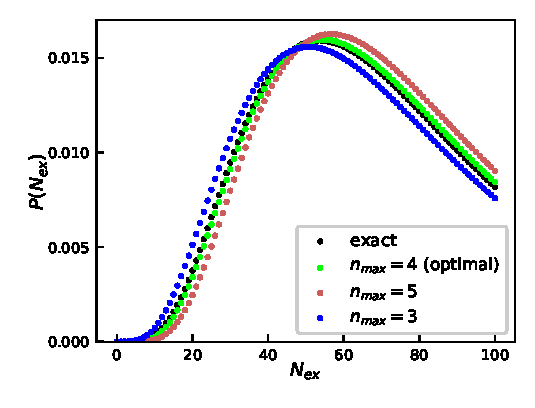
\includegraphics{fig1.eps}
\caption{Comparison of exact  distribution $P(N_{ex})$ and discretized 
classical fields distribution $P_{cl}(N_{ex})$ obtained for different values of 
cutoff parameter $n_{max}$. The inverse temperature equals $\beta=0.03625$. We 
observe that cutoff obtained from relation~\eqref{eq:cutoff} provides the best 
agreement between curves.}
\label{fig:comp}
\end{figure}

Comparing $P(N_{ex})$ and $P_{cl}(N_{ex})$ leads us to the conclusion that 
cutoff parameter should be determined from following relation
\begin{equation}
\label{eq:cutoff}
n_{max} = \sqrt{C k_{\textit{B}} T}
\end{equation}
with $C=0.58$. 

With a suitable cutoff we are able to obtain average number of atoms in the 
condensate and its fluctuations as a function of temperature. We use two 
approaches described in Sec.~\ref{model}. Our results 
are presented in Fig.~\ref{fig:stat}.
    
Initial conditions for the evolution were chosen from the set of states 
generated by the Monte Carlo algorithm in such a way  that the energy of the 
state was the closest to the equilibrium value and the momentum was closest to 
zero. Two states randomly selected in this way in principle  may differ in 
values of other constants of motion, which in turn may lead to somewhat 
different values of time-averaged quantities. However, we have observed that 
for sufficiently strong interactions time averaged fluctuations and populations 
do not depend on the choice of initial conditions provided the energies 
and momenta are the same.
\begin{figure*}[!]
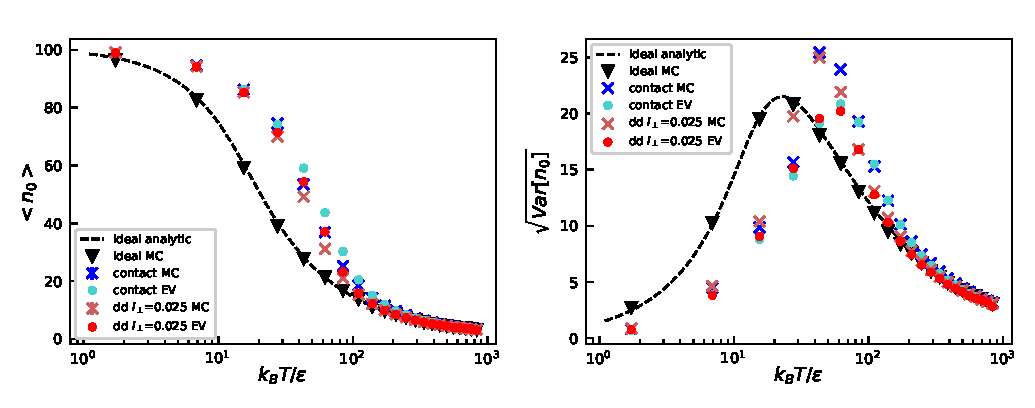
\includegraphics{fig2.eps}
\caption{Average occupation of the condensate (left) and its fluctuations 
(right) as a function of temperature. We have obtained results for ideal and 
interacting gas with $g=1.0$. For the ideal gas we are able to reproduce with 
MC simulations exact analytic results calculated in canonical ensemble. We 
compare contact interactions and dipolar with $l_{\perp}=0.025$. Note that 
fluctuations obtained in time evolution are smaller than those from MC 
simulations. Contrary to 1D harmonic trap~\cite{Bienias2011b}, depletion with 
temperature of interacting gas is slower than in case of the ideal gas.}
\label{fig:stat}
\end{figure*}

Microcanonical ensemble, as well as our equations, do not involve 
temperature - the temperature is not a control parameter of microcanonical 
ensemble. Thus, the temperature in the case of time evolution should not be 
seen as a physical parameter, but rather as an indicator telling us that 
the evolution was performed for the  occupation of modes and energy 
characteristic for a system in equilibrium at the temperature $T$.
    
The interaction strength used for simulations was $g=1.0$. In order to check 
whether this value corresponds to the regime of weakly interacting gas, we have 
calculated quantum depletion of the condensate at $T=0$ within the standard 
Bogoliubov approximation. The depletion turned out to be around 14 percent.

\subsection{Coherence length}
The problem of phase coherence and closely related momentum distribution of the 
gas in 1D harmonic trap was investigated both experimentally~\cite{Richard2003} 
and theoretically~\cite{Kadio2005}.

Due to dimensionality of our system, for high enough temperatures, we enter the 
regime where so-called quasicondensation occurs. Quasicondensation refers to 
the situation where there is no dominant eigenvalue of single-particle density 
matrix. In other words, there is more than one mode with macroscopic 
population. This phenomenon is clearly visible in exact results concerning the 
ideal gas and occurs for repulsive gas as well. In this paragraph we look at 
the normalized correlation function (brackets $\langle \cdot \rangle$ denote 
canonical ensemble average)
\begin{equation}
\label{eq:correlation}
g_1(x-x') = \frac{\langle \hat{\psi}^{\dag}(x) \hat{\psi}(x') \rangle}
{\sqrt{\langle |\hat{\psi}(x)|^2 \rangle \langle |\hat{\psi}(x')|^2 \rangle}}
\end{equation}
with a special attention given to coherence length measuring the rate of decay 
of the function~\eqref{eq:correlation}. Correlation function depends heavily on 
occupations of higher energy modes, that is why, due to quasicondensation, we 
no longer can rely on criterion~\eqref{eq:cutoff} which was established by 
matching distributions that focus on occupation of the ground state only and in 
a sense do not take into account the distribution of higher modes. 
Therefore, new formula for cutoff is needed.
\begin{figure}[h]
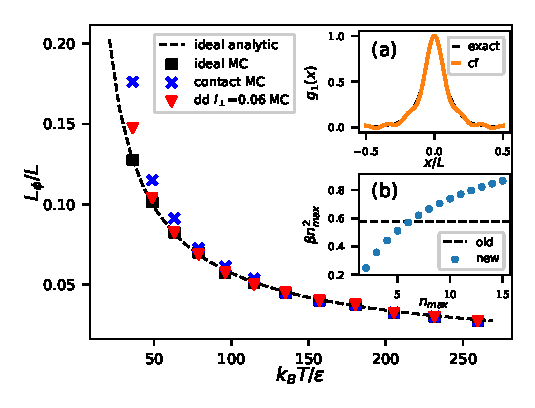
\includegraphics{fig3.eps}
\caption{Coherence length as a function of temperature for $g=0.2$. We compare 
results for contact and dipolar interactions with $l_{\perp}=0.06$. With new 
values of cutoff parameter $n_{max}$ obtained by matching HWHM of exact and 
classical fields correlation function of the ideal gas $(a)$ we are able to 
reproduce with MC simulations coherence length calculated from analytic 
formulas. The lower inset $(b)$ presents comparison of cutoff~\eqref{eq:cutoff} 
and new cutoff suited for coherence length. From relation~\eqref{eq:cutoff} we 
see that $\beta n_{max}^2=0.58=\text{const}$ contrary to values of $n_{max}$ 
obtained to match HWHMs.}
\label{fig:coherence}
\end{figure}

Again, we consider noninteracting gas within the framework of canonical 
ensemble and calculate correlation function in exact treatment (with discrete 
occupations of states) and in classical fields approximation (for details see 
the Appendix). We have decided to measure the coherence length $L_{\phi}$ by 
half width at half maximum (HWHM) of function~\eqref{eq:correlation}. Cutoff is 
chosen to match coherence length obtained from correlation function in exact 
treatment and in classical fields approximation (see 
Fig.~\ref{fig:coherence}$(a)$). New values of cutoff parameter in relation to 
the old ones (from formula~\eqref{eq:cutoff}) are presented in 
Fig.~\ref{fig:coherence}$(b)$. We study the decay of coherence length with 
temperature (see Fig.~\ref{fig:coherence}).
It is interesting to notice that correlation function of the ideal gas (see 
Fig.~\ref{fig:coherence}$(a)$) is fairly smooth at the neighbourhood of zero 
and does not display cusp as it is in the case of gas in harmonic trap
~\cite{Kadio2005}. The reason can be attributed to faster decay of occupations 
of subsequent energy levels which serve a role of coefficients in a expression 
for correlation function (for details see the Appendix). The difference is 
caused by different dependence of energy on quantum number which is linear for 
harmonic trap and quadratic in our system.

\section{The attractive gas}\label{attractive}
Now we turn our attention to the attractive gas. This time even in 
low-temperature regime we expect quasicondensate. We observe that in results of 
Monte Carlo simulations, where even for very weak interactions and very low 
temperature, condensate population is far from 100 percent. Moreover, we expect 
bright solitons in desity profile of the gas.

\subsection{The cutoff}
Because of quasicondensation for the attractive gas, we can no longer extend 
our ideal gas cutoff criterion~\eqref{eq:cutoff}. The choice of the cutoff 
should be modified.
    
We start with finding an estimate of the ground state of attractive gas of $N$ 
particles. We employ two methods: analytical approximation and numerical 
algorithm. One can expect that the wave function of the ground state will take 
a localized shape due to the attractive interactions. Basing on this assumption 
we take the wave function of the following form
\begin{equation}\label{eq:optimal}
\Psi(x_1 , \ldots , x_N) = \prod_{j=1}^N \varphi(x_j), \hspace{0.16cm} 
\varphi(x) = \frac{1}{\sqrt{\sqrt{\pi} \lambda}} 
e^{-\frac{1}{2}(\frac{x}{\lambda})^2}
\end{equation}
with a free parameter $\lambda$ describing the width of the wave function. 
Such a form of the ansatz does not take the periodicity into account, therefore 
we expect it to describe our system well only if $\lambda$ is small enough. We 
then minimize the energy in this state with respect to $\lambda$. For contact 
interactions, the interaction energy can be computed analytically. The total 
energy reaches minimum for $\lambda=\frac{1}{\sqrt{2} \pi^{3/2} |g| (N-1)}$ 
and equals
\begin{equation}
E_{\delta} = -\frac{1}{4} \pi g^2 (N-1)^2 N
\end{equation}
However, it is not possible to analytically solve the dipole-dipole interaction 
and thus in this case the energy was computed numerically and the minimimum was 
found numerically (for broader analysis of density distribution see
~\cite{Adhikari2012}). That is the reason why in Fig.~\ref{fig:reproducing} for 
contact interactions we draw continous line, but for dipolar ones we have 
restricted ourselves to the values of interaction strength used to perform MC 
simulations.
   
Our goal was to the modify cutoff in such a way that Monte Carlo simulations at 
very low temperature reproduce the energy and the width of the optimal state 
(see Fig.~\ref{fig:reproducing}). This approach is similar to
~\cite{Bienias2011c} and can be expressed in formula
\begin{equation}
\label{eq::cutoff2}
n_{max} = \sqrt{C k_{\textit{B}} T} + n(g)
\end{equation}
where $n(g)$ is the number of mode pairs we have to add to reproduce the 
optimal state. We emphasize that extension of above formula to high 
temperatures is not obvious.
\begin{figure}
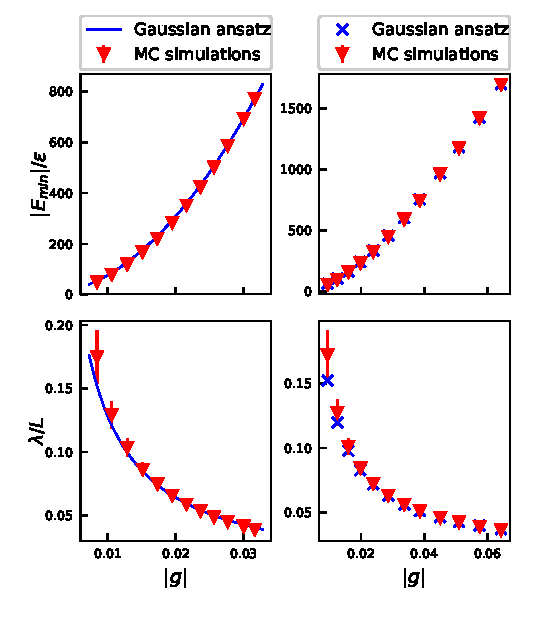
\includegraphics{fig4.eps}
\caption{Results of reproducing the optimal state from Gaussian ansatz
~\eqref{eq:optimal} with MC simulations. The left panels present data for 
contact interactions, whereas the right panels correspond to the dipolar 
interaction with $l_{\perp}=0.025$. The first row compares average energy at 
very low temperature $\beta=0.58$ obtained using cutoff criterion
~\eqref{eq::cutoff2} with energy of optimal state with the same value of $g$. 
The values of interaction strength for which the MC simulations were performed 
correspond to the values of $n(g)=1, \ldots , 12$. The second row presents 
comparison between the width of the optimal state and average width from MC 
simulations. Note the differences for wide states with large $\lambda$.}
\label{fig:reproducing}
\end{figure}

\subsection{Random walk}
It is clear that the many-body Hamiltonian we consider commutes with the 
rotation generator. For this reason, the multi-particle wave function of the 
ground state should not change under rotations. However, when measuring 
positions of individual particles, one should rather expect localized 
Gaussian-like shape with well-defined position of maximum as a result. Of 
course, no point on the circle is distuinguished, so in the series of 
measurements, we should see uniform distribution of positions of the maximum.
    
The phenomenon of spontaneous symmetry breaking via measurement was understood 
over twenty years ago in the case of interference of two condensates
~\cite{Javanainen1996,Andrews1997} and more recently, for excited state of 1D 
repulsive gas in the ring geometry~\cite{Syrwid2015}.
\begin{figure}[h]
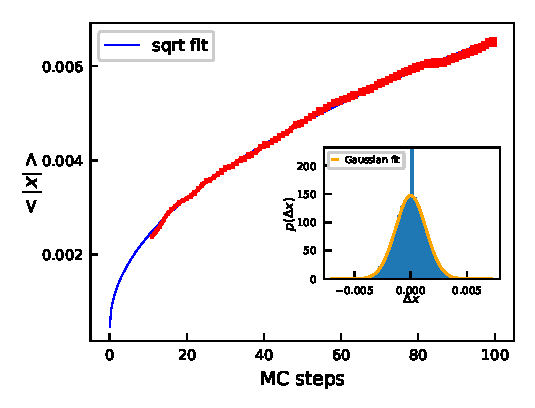
\includegraphics{fig5.eps}
\caption{Average distance traveled by the wave packet maxima and a histogram of 
the shift in its position after a single MC step with corresponding function 
fits - $\sqrt{n/a}+b$ and a normal distribution respectively. Note the spike 
in the histogram at $\Delta x=0$, the fit was done ignoring this spike. 
Interactions used for simulations were contact with interaction strength 
$g=-0.0152$.}
\label{fig:randomwalk}
\end{figure}
    
We are able to somehow relate these remarks about breaking the rotational 
symmetry to results from MC simulations and time evolution. Firstly, we take 
the Metropolis algorithm and treat each consecutive sample as an element of 
a discrete time sequence. Then, we show that the peak of the wave profile 
exhibits Brownian motion properties (such as mean distance after $n$ time steps 
behaves like $\sqrt{n}$; each consecutive pair of changes in positions is not 
correlated). So, it is indeed Markovian random walk, despite the spike in the 
histogram presented in Fig.~\ref{fig:randomwalk}. The spike is a delta-like 
addition to otherwise normal distrubution of position shifts. It is a byproduct 
of the Metropolis algorithm and more precisely, it is caused by the rejection 
rate of the new sets of alphas. The coefficient of the delta-like factor - the 
probability that there will be no change in a position caused by the rejection 
of a new set of alphas - directly corresponds and is equal to the rejection 
probability of the algorithm. By default, we optimize the rejection probability 
to be $0.5$ for fastest thermalization. It is interesting to note that within 
the classical fields approximation, individual realization of the field breaks 
symmetry and thus corresponds to a single measurement. The whole ensemble 
restores the rotational symmetry because samples do not distuinguish any point 
on the circle.
    
Then, we provided the equations~\eqref{eq:eqs} with initial conditions 
generated by MC algorithm for parameters guarrenteeing presence of bright 
solitons. The shape of the soliton was preserved during time evolution. We 
analyzed the positions of peak obtained in equal time steps. It turns out that 
the distribution of jump's length is Gaussian, but due to correlation between 
length of two consecutive jumps (peak tends to travel in one direction for 
quite a long time) we did not observe characteristic $\sqrt{t}$ behavior 
of a mean distance.
\begin{figure}[h]
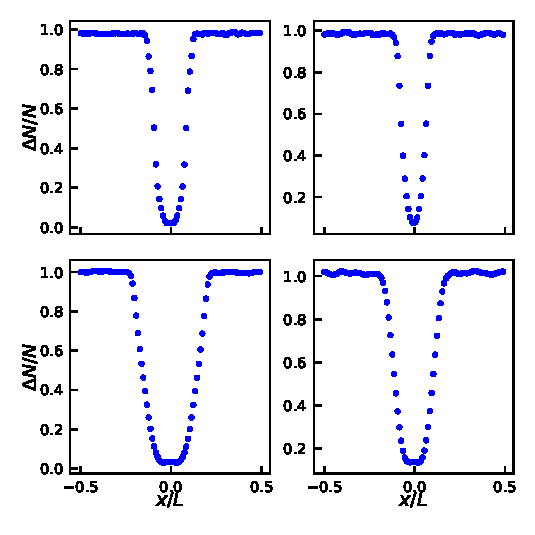
\includegraphics{fig6.eps}
\caption{Local density fluctuations. The left panels present data for 
$\beta=0.58$, whereas for the right panels we have $\beta=0.0644$. We compare 
results for contact interaction (upper row) and dipolar with $l_{\perp}=0.05$ 
(lower row) with equal interaction strength $g=-0.0439$. The trap was divided 
into 101 bins.}
\label{fig:localfluc}
\end{figure}

\subsection{Local density fluctuations}
The last issue of attractive gas is the problem of local density fluctuations. 
For every sample generated by Monte Carlo simulation, we consider its density 
profile. Every density profile corresponds to a different position of the 
soliton. That is why using bins with positions fixed relatively to the ring 
would not lead us to reveal any structure in the distribution of density 
fluctuations across bins. We use other approach in which for every sample we 
start with determining the position of the center of mass (CM) of our system. 
Then we divide the ring into bins with respect to the position of the CM. 
Finally, we collect data from all samples generated with MC algorithm and 
measure the variance of the number of atoms in each bin 
(see Fig.~\ref{fig:localfluc}).

\section{Summary}\label{summary}
We have thoroughly studied statistical properties of Bose gas confined to a 
ring trap, both for contact and dipolar interactions. Our results concern 
problems that are already accesible for experimental verification in harmonic 
traps. For repulsive gas, not only did we concentrated on average value and 
fluctuations of the zero momentum component, but also investigated the 
coherence length as a function of temperature, the quantity which depends on 
occupuation of higher energy modes. We have shown that with a proper criterion 
for the cutoff, classical fields approximation can tackle not only problems 
connected with occupation of the lowest energy mode, but can also be useful in 
the quasicondensation regime, in particular to study coherence length and local 
density fluctuations in the case of attractive gas.

For gas with attractive interactions, apart from local density fluctuations we 
have analyzed the evolution of classical field throughout the Metropolis 
algorithm and the Heisenberg equation of motion. Our observations of the 
evolution of density profile lead us to conclusion that consecutive positions 
of the soliton display the same properties as one would expect from series of 
measurements of particles on the ring and therefore support interpretation that 
single realization of the classical field corresponds to a single measurement.
\begin{acknowledgments}
We thank K. Pawłowski for enlightening discussions and P. Grochowski for 
careful reading of the manuscript. Authors were supported by (Polish) National 
Science Center Grant 2015/19/B/ST2/02820. Center for Theoretical Physics PAN is 
a member of KL FAMO. This research was supported in part 
by PLGrid Infrastructure.    
\end{acknowledgments}

M.K. and M.Ł. contributed equally to this work.

\appendix
\onecolumngrid

\section{Partition function of the ideal gas}
We consider a system of $N$ particles on the ring in thermal contact with a 
heat reservoir at the temperature $T$. We start with calculating canonical 
partition function. By $n_i$ and $E_i$ we denote occupation and energy of 
$i$th state. We introduce shift of the energy scale such that all energies are 
positive. Partition function takes the form
\begin{equation}
Z_N(\beta) = \sum_{n_{-\infty}=0}^{\infty} \ldots \sum_{n_{\infty}=0}^{\infty} 
e^{-\beta \sum_j E_j n_j} \; \delta_{N, \sum_j n_j}.
\end{equation}
We use  integral representation of the Kronecker delta
\begin{equation}
\delta_{N, \sum_j n_j} = \frac{1}{2 \pi} \int_0^{2 \pi} \mathrm{d} \xi \; 
e^{i \xi \big(N-\sum_j n_j\big)}.
\end{equation}
After changing order of summation and integration, we are able to evaluate 
sums. Note that in case of atoms on the ring all energies except $E_0$ are 
double-degenerated ($E_i=E_{-i}$). We arrive at
\begin{equation}
Z_N(\beta) = \frac{1}{2 \pi} \int_0^{2 \pi} \mathrm{d} \xi \; e^{i \xi N} 
\prod_{j=-\infty}^{\infty} \frac{1}{1-e^{-(i \xi+\beta E_j)}} = \frac{1}{2 \pi} 
\int_0^{2 \pi} \mathrm{d} \xi \; \frac{e^{i \xi N}}{1-e^{-(i \xi+\beta E_0)}} 
\prod_{j=1}^{\infty} \frac{1}{(1-e^{-(i \xi+\beta E_j)})^2}.
\end{equation}
In the next step we perform variable change $z=e^{i \xi}$ and end up with 
integrating function $f(z)=\frac{z^N}{z-e^{-\beta E_0}} \prod_{j=1}^{\infty} 
\frac{z^2}{(z-e^{-\beta E_j})^2}$ over the unit circle. We employ the residue 
theorem method. For $z=e^{-\beta E_0}$ there is a first-order pole and in 
$z=e^{-\beta E_k}$, $k \neq 0$ we have poles of order 2. We finally obtain 
partition function 
\begin{equation}
\label{eq:pfexact}
\begin{split}
Z_N(\beta) &= e^{-\beta E_0 N} \prod_{j=1}^{\infty} 
\frac{1}{(1-e^{-\beta (E_j-E_0)})^2} + \\ 
&+ \sum_{j=1}^{\infty} \frac{e^{-\beta E_j N}}{1-e^{-\beta (E_0-E_j)}} 
\prod_{\substack{k=1 \\ k \neq j}}^{\infty} 
\frac{1}{(1-e^{-\beta (E_k-E_j)})^2} \Bigg(N + 1 + 
\frac{1}{1-e^{-\beta (E_j-E_0)}} + 2\sum_{\substack{l=1 \\ l \neq j}}^{\infty} 
\frac{1}{1-e^{-\beta (E_j-E_l)}} \Bigg).
\end{split}
\end{equation}

\subsection*{Classical fields}
Now we calculate partition function in the classical fields description of 
particles on the ring. It means that we have to introduce cutoff parameter $n$ 
and occupations of modes are no longer discrete $n_i=|\alpha _i |^2$. Partition 
function can be written in a form
\begin{equation}
Z_N^{cl}(\beta) = \int \frac{\mathrm{d}^2 \alpha_{-n}}{\pi} \ldots \int 
\frac{\mathrm{d}^2 \alpha_n}{\pi} \; e^{- \beta \sum_j E_j |\alpha_j|^2} 
\delta \bigg(N-\sum_{j=-n}^n |\alpha_j|^2 \bigg).
\end{equation}
We use  the Dirac delta representation
\begin{equation}
\delta \bigg(N-\sum_{j=-n}^n |\alpha_j|^2 \bigg) = \frac{1}{2 \pi} 
\int_{-\infty}^{\infty} \mathrm{d} \xi \; 
e^{i \xi \big(N-\sum_j |\alpha_j|^2 \big)}.
\end{equation}
Hence
\begin{equation}
Z_N^{cl}(\beta) = \frac{1}{2 \pi} \int_{-\infty}^{\infty} \mathrm{d} \xi \; 
e^{i \xi N} \, I_{-n} \ldots I_n, \qquad I_k = \int 
\frac{\mathrm{d}^2 \alpha_{k}}{\pi} \, e^{-|\alpha_k|^2(\beta E_k+i \xi)} = 
\frac{1}{\beta E_k+ i \xi}.
\end{equation}
All energies except $E_0$ are double-degenerated ($E_i=E_{-i}$)
\begin{equation}
\label{eq:pfclint}
Z_N^{cl}(\beta) = \frac{1}{2 \pi} \int_{-\infty}^{\infty} \mathrm{d} \xi \; 
e^{i \xi N} \prod_{j=-n}^{n} \frac{1}{\beta E_j+i \xi} = \frac{(-1)^n}{2 \pi i} 
\int_{-\infty}^{\infty} \mathrm{d} \xi \; e^{i \xi N} 
\frac{1}{\xi- i \beta E_0} \prod_{j=1}^n \frac{1}{(\xi - i \beta E_j)^2}.
\end{equation}
To calculate integral~\eqref{eq:pfclint} we consider function 
$g(z)=\frac{e^{i z N}}{z-i \beta E_0} \prod_{j=1}^n 
\frac{1}{(z-i \beta E_j)^2}$ and integrate it over semicircle in the upper 
half-plane using the residue theorem (integral over arc vanishes in the limit 
of infinite radius). For $z=i \beta E_0$ there is a pole of order 1, and for 
$z=i \beta E_k$ , $k \neq 0$ we have poles of order 2. 
Partition function follows from the residue theorem formula
\begin{equation}
\label{eq:pfclass}
\begin{split}
Z_N^{cl}(\beta) &= e^{-\beta E_0 N} \prod_{j=1}^n 
\frac{1}{(\beta E_j-\beta E_0)^2}+\\&+\sum_{j=1}^n 
\frac{e^{-\beta E_j N}}{\beta E_0-\beta E_j} 
\prod_{\substack{k=1 \\ k \neq j}}^n \frac{1}{(\beta E_k -\beta E_j)^2} 
\Bigg(N + \frac{1}{\beta E_j-\beta E_0} + 2\sum_{\substack{l=1 \\ l \neq j}}^n 
\frac{1}{\beta E_j-\beta E_l} \Bigg).
\end{split}  
\end{equation}

\section{Probability distribution}
We are interested in a probability distribution $P(N_{ex})$  of having $N_{ex}$ 
atoms excited and $N_0=N-N_{ex}$ occupying the ground state. To obtain 
the distibution we use simple formula~\cite{Weiss1997}
\begin{equation}
\label{eq:pnex}
P(N_{ex}) = \frac{Z_{N_{ex}}}{Z_N}
\end{equation}
where $Z_{N_{ex}}$ is partition function calculated for situation where 
$N_{ex}$ atoms are excited and the rest occupy the ground state. We calculate 
$Z_{N{ex}}$ following the same steps as in the case of partition function
~\eqref{eq:pfexact}. Using formula~\eqref{eq:pnex} and setting $E_0=0$ gives us 
\begin{equation}
P(N_{ex}) = \frac{\sum_{j=1}^{\infty} e^{-\beta E_j N_{ex}} 
\prod_{\substack{k=1 \\ k \neq j}}^{\infty} \frac{1}{(1-e^{-\beta(E_k-E_j)})^2} 
\bigg(N_{ex} + 1 + 2\sum_{\substack{l=1 \\ l \neq j}}^{\infty} 
\frac{1}{1-e^{-\beta(E_j-E_l)}} \bigg)}
{\prod _{j=1}^{\infty} \frac{1}{(1-e^{-\beta E_j})^2} - 
\sum_{j=1}^{\infty}\frac{e^{-\beta E_j N}}{e^{ \beta E_j}-1} 
\prod_{\substack{k=1 \\ k \neq j}}^{\infty} \frac{1}{(1-e^{-\beta(E_k-E_j)})^2} 
\bigg(N + 1 + \frac{1}{1-e^{-\beta E_j}} + 
2\sum_{\substack{l=1 \\ l \neq j}}^{\infty} 
\frac{1}{1-e^{-\beta(E_j-E_l)}} \bigg)}.
\end{equation}

\subsection*{Classical fields}
Again we use formula~\eqref{eq:pnex} with $Z^{cl}_{N_{ex}}$ calculated 
similarly as~\eqref{eq:pfclass} and obtain 
\begin{equation}
P_{cl}(N_{ex}) = \frac{\sum_{j=1}^n e^{-\beta E_j N_{ex}} 
\prod_{\substack{k=1 \\ k \neq j}}^n \frac{1}{(\beta E_k-\beta E_j)^2} 
\bigg(N_{ex} + 2\sum_{\substack{l=1 \\ l \neq j}}^n 
\frac{1}{\beta E_j-\beta E_l}\bigg)}
{\prod_{j=1}^n \frac{1}{(\beta E_j)^2} - 
\sum_{j=1}^n \frac{e^{-\beta E_j N}}{\beta E_j} 
\prod_{\substack{k=1 \\ k \neq j}}^n \frac{1}{(\beta E_k-\beta E_j)^2}
\bigg(N + \frac{1}{\beta E_j} + 2\sum_{\substack{l=1 \\ l \neq j}}^n 
\frac{1}{\beta E_j-\beta E_l}\bigg)}.
\end{equation}

\section{Correlation function}
In order to calculate coherence length we need to obtain  the function 
$\langle \hat{\psi}^{\dag}(x) \hat{\psi}(x') \rangle$, where brackets 
$\langle \cdot \rangle$ denote canonical ensemble average. We decompose atomic 
field in momentum basis
\begin{equation}
\label{eq:atomic}
\hat{\psi}(x) = \sum _q \frac{1}{\sqrt{L}} \, \hat{a}_q \, e^{i q x}
\end{equation}
and write
\begin{equation}
\langle \hat{\psi}^{\dag}(x) \hat{\psi}(x') \rangle = \frac{1}{L} \sum_{q,q'} 
\langle \hat{a}_q^{\dag} \hat{a}_{q'} \rangle \, e^{i (q'x'-qx)} = \frac{1}{L} 
\sum_{q} \langle n_q \rangle \, e^{i q(x'-x)} = \frac{1}{L} \bigg(\langle n_0 
\rangle + 2\sum_{q=1}^{\infty} \langle n_q \rangle \, \cos \big(q(x-x')\big) 
\bigg).
\end{equation}
Above we used the fact that $\langle \hat{a}_q^{\dag} \hat{a}_{q'} \rangle = 
\delta_{q,q'} \langle n_q \rangle$ and $\langle n_q \rangle = \langle n_{-q} 
\rangle$. As we see, the whole calculation boils down to obtaining average 
occupation of all modes. This can be done in a similar way as the partition 
function (using the residue theorem) or simply by differentiating expression 
for partition function~\eqref{eq:pfexact}. For $q=0$ we have
\begin{equation}
\label{eq:avzero}
\langle n_0 \rangle = \frac{1}{Z_N(\beta)} \sum_{j=0}^{\infty} 
e^{-\beta E_j (N-1)} \prod_{\substack{k=0 \\ k \neq j}}^{\infty} 
\frac{1}{(1-e^{-\beta (E_k-E_j)})^2} 
\Bigg(N + 2\sum_{\substack{l=0 \\ l \neq j}}^{\infty} 
\frac{1}{1-e^{-\beta (E_j-E_l)}} \Bigg),
\end{equation}
whereas for $q \neq 0$ we obtain
\begin{equation}
\begin{split}
\langle n_q \rangle &= \frac{1}{Z_N(\beta)} \Bigglb (\frac{1}{e^{\beta E_q}-1} 
\prod_{j=1}^{\infty} \frac{1}{(1-e^{-\beta E_j})^2} - 
\sum_{\substack{j=1 \\ j \neq q}}^{\infty} 
\frac{e^{-\beta E_j N}}{e^{\beta E_j}-1} \frac{1}{e^{\beta (E_q-E_j)}-1} 
\prod_{\substack{k=1 \\ k \neq j}}^{\infty} 
\frac{1}{(1-e^{-\beta (E_k-E_j)})^2} \\ 
& \times \Bigg(N + \frac{1}{1-e^{-\beta (E_j-E_q)}} + 
\frac{1}{1-e^{-\beta E_j}} + 2\sum_{\substack{l=1 \\ l \neq j}}^{\infty} 
\frac{1}{1-e^{-\beta (E_j-E_l)}} \Bigg) - 
\frac{e^{-\beta E_q N}}{e^{\beta E_q}-1} 
\prod_{\substack{j=1 \\ j \neq q}}^{\infty} 
\frac{1}{(1-e^{-\beta (E_j-E_q)})^2} \\ 
& \times \Bigg(\frac{N (N+1)}{2} + \frac{N}{(1-e^{-\beta E_q})^2} + 
2\Big(N + 1 + \frac{1}{1-e^{-\beta E_q}} \Big) 
\sum_{\substack{k=1 \\ k \neq q}}^{\infty} \frac{1}{1-e^{-\beta (E_q-E_k)}} + 
\sum_{\substack{k=0 \\ k \neq q}}^{\infty} \frac{1}{(1-e^{-\beta (E_q-E_k)})^2} 
+ \\ 
& + 2\sum _{\substack{k,k'=1 \\ k,k' \neq q \\ k \neq k'}}^{\infty} 
\frac{1}{(1-e^{-\beta (E_q-E_k)}) (1-e^{-\beta (E_q-E_{k'})})} + \frac{1}{2} 
\sum_{\substack{k=1 \\ k \neq q}}^{\infty} 
\frac{1}{\text{sinh}^2 \big(\frac{1}{2} \beta (E_q-E_k) \big)} - 
\frac{N}{4} \frac{1}{\text{sinh}^2 \big(\frac{1}{2} \beta E_q \big)} 
\Bigg) \Biggrb ).
\end{split}
\end{equation}

\subsection*{Classical fields}
Replacing annihilation operators with complex amplitudes in expression
~\eqref{eq:atomic} leads to classical version of atomic field. From that 
follows the correlation function
\begin{equation}
\langle \psi^{*}(x) \psi(x') \rangle = \frac{1}{L} \sum_{q,q'} \langle 
\alpha_q^* \alpha_{q'} \rangle \, e^{i (q'x'-qx)} = \frac{1}{L} \sum_{q} 
\langle |\alpha_q|^2 \rangle \, e^{i q(x'-x)} = \frac{1}{L} 
\bigg(\langle |\alpha_0|^2 \rangle + 2\sum_{q=1}^{\infty} 
\langle |\alpha_q|^2 \rangle \, \cos \big(q(x-x')\big) \bigg).
\end{equation}
Using similar methods as in the case of partition function (the residue 
theorem) or by differentiation of~\eqref{eq:pfclass} we obtain for $q=0$
\begin{equation}
\langle |\alpha_0|^2 \rangle = \frac{1}{Z_N^{cl}(\beta)} 
\sum_{j=0}^n e^{-\beta E_j N} \prod_{\substack{k=0 \\ k \neq j}}^n 
\frac{1}{(\beta E_k - \beta E_j )^2} \Bigg(N + 
2\sum_{\substack{l=0 \\ l \neq j}}^n \frac{1}{\beta E_j-\beta E_l} \Bigg),
\end{equation}
for $q \neq 0$ we have
\begin{equation}
\begin{split}
\langle |\alpha _q|^2 \rangle &= \frac{1}{Z_N^{cl}(\beta)} 
\Bigglb (\frac{1}{\beta E_q} \prod_{j=1}^n \frac{1}{(\beta E_j)^2} - 
\sum_{\substack{j=1 \\ j\neq q}}^n \frac{e^{-\beta E_j N}}{\beta E_j} 
\frac{1}{\beta E_q-\beta E_j} \prod_{\substack{k=1 \\ k \neq j}}^n 
\frac{1}{(\beta E_k -\beta E_j)^2} \\ 
& \times \Bigg(N + \frac{1}{\beta E_j -\beta E_q} + \frac{1}{\beta E_j} + 
2\sum_{\substack{l=1 \\ l \neq j}}^n \frac{1}{\beta E_j -\beta E_l} \Bigg) - 
\frac{e^{-\beta E_q N}}{\beta E_q} \prod_{\substack{j=1 \\ j \neq q}}^n 
\frac{1}{(\beta E_q-\beta E_j)^2} \\ 
& \times \Bigg(\frac{N^2}{2} + \frac{N}{\beta E_q} + \frac{1}{(\beta E_q)^2} + 
2\Big(N + \frac{1}{\beta E_q} \Big) \sum_{\substack{k=1 \\ k \neq q}}^n 
\frac{1}{\beta E_q -\beta E_k} + \\ 
& + 2\sum_{\substack{k,k'=1 \\ k,k' \neq q \\ k \neq k'}}^n 
\frac{1}{(\beta E_q- \beta E_k) (\beta E_q- \beta E_{k'})} + 
3\sum_{\substack{k=1 \\ k \neq q}}^n \frac{1}{(\beta E_q-\beta E_k)^2} 
\Bigg) \Biggrb ).
\end{split}
\end{equation}

\section{Fluctuations}
The variance of population of the condensate is equal 
$\text{Var}(n_0)=\langle n_0^2 \rangle -\langle n_0 \rangle ^2$. We have 
already found average population~\eqref{eq:avzero}, the remaining component is
\begin{equation}
\begin{split}
\langle n_0 ^2 \rangle &= \frac{1}{Z_N(\beta)} \Bigglb ( \,\prod_{j=1}^{\infty} 
\frac{1}{(1-e^{-\beta E_j})^2} \Bigg(N^2 - 2 (2N+1)\sum_{k=1}^{\infty} 
\frac{1}{e^{\beta E_k}-1} + 4\sum_{\substack{k,k'=1 \\k \neq k'}}^{\infty} 
\frac{1}{(e^{\beta E_k}-1)(e^{\beta E_{k'}}-1)} + \\ 
& + 2\sum_{k=1}^{\infty} \frac{1}{(e^{\beta E_k}-1)^2} + 
\sum_{k=1}^{\infty} \frac{1}{\text{sinh}^2(\frac{1}{2} \beta E_k)} \Bigg) - 
\sum_{j=1}^{\infty} \frac{e^{-\beta E_j N}}{1-e^{-\beta E_j}} 
\prod_{\substack{k=0 \\ k \neq j}}^{\infty} \frac{1}{(1-e^{-\beta(E_k-E_j)})^2} 
\\ 
& \times \Bigg(1 + \Big(e^{\beta E_j}+1\Big) \bigg(N + 
\frac{1}{e^{\beta E_j}-1} + 2\sum_{\substack{l=0 \\ l \neq j}}^{\infty} 
\frac{1}{1-e^{-\beta(E_j-E_l)}} \bigg) \Bigg) \Biggrb ).
\end{split}
\end{equation}

\twocolumngrid
\bibliography{bibliography.bib}
\end{document}